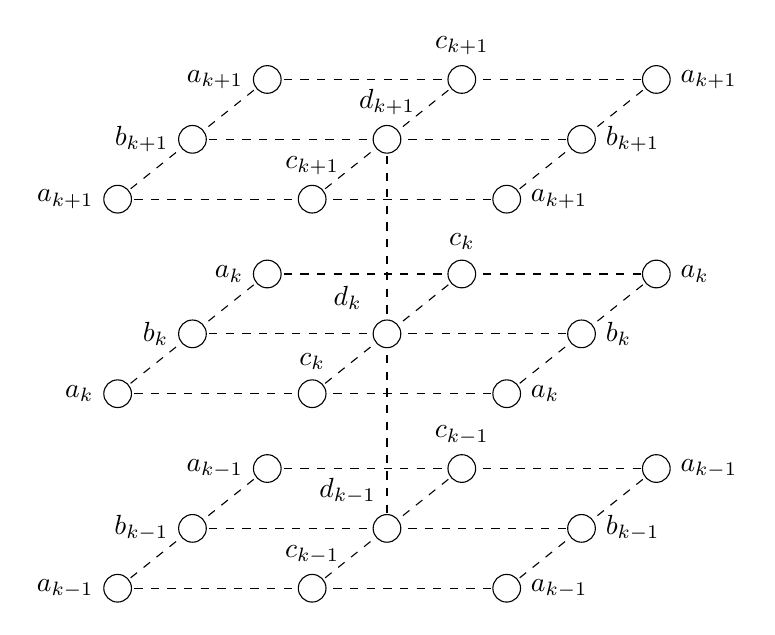
\begin{tikzpicture}[xscale=1.9,yscale=1.9]
\def\length{1.3};\def\offsetx{.5};\def\offsety{.4};\def\vertoffset{-1.3};
\coordinate (top_1) at (0,0);
\coordinate (top_2) at (\length,0);
\coordinate (top_3) at (2*\length,0);
\coordinate (top_4) at (\offsetx,\offsety);
\coordinate (top_5) at (\length+\offsetx,\offsety);
\coordinate (top_6) at (2*\length+\offsetx,\offsety);
\coordinate (top_7) at (2*\offsetx,2*\offsety);
\coordinate (top_8) at (\length+2*\offsetx,2*\offsety);
\coordinate (top_9) at (2*\length+2*\offsetx,2*\offsety);

\coordinate (mid_1) at (0,\vertoffset);
\coordinate (mid_2) at (\length,\vertoffset);
\coordinate (mid_3) at (2*\length,\vertoffset);
\coordinate (mid_4) at (\offsetx,\offsety+\vertoffset);
\coordinate (mid_5) at (\length+\offsetx,\offsety+\vertoffset);
\coordinate (mid_6) at (2*\length+\offsetx,\offsety+\vertoffset);
\coordinate (mid_7) at (2*\offsetx,2*\offsety+\vertoffset);
\coordinate (mid_8) at (\length+2*\offsetx,2*\offsety+\vertoffset);
\coordinate (mid_9) at (2*\length+2*\offsetx,2*\offsety+\vertoffset);

\coordinate (bot_1) at (0,2*\vertoffset);
\coordinate (bot_2) at (\length,2*\vertoffset);
\coordinate (bot_3) at (2*\length,2*\vertoffset);
\coordinate (bot_4) at (\offsetx,\offsety+2*\vertoffset);
\coordinate (bot_5) at (\length+\offsetx,\offsety+2*\vertoffset);
\coordinate (bot_6) at (2*\length+\offsetx,\offsety+2*\vertoffset);
\coordinate (bot_7) at (2*\offsetx,2*\offsety+2*\vertoffset);
\coordinate (bot_8) at (\length+2*\offsetx,2*\offsety+2*\vertoffset);
\coordinate (bot_9) at (2*\length+2*\offsetx,2*\offsety+2*\vertoffset);


\draw[dashed] (top_1)--(top_7);
\draw[dashed] (top_2)--(top_8);
\draw[dashed] (top_3)--(top_9);
\draw[dashed] (top_1)--(top_3);
\draw[dashed] (top_4)--(top_6);
\draw[dashed] (top_7)--(top_9);

\draw[dashed] (mid_1)--(mid_7);
\draw[dashed] (mid_2)--(mid_8);
\draw[dashed] (mid_3)--(mid_9);
\draw[dashed] (mid_1)--(mid_3);
\draw[dashed] (mid_4)--(mid_6);
\draw[dashed] (mid_7)--(mid_9);

\draw[dashed] (bot_1)--(bot_7);
\draw[dashed] (bot_2)--(bot_8);
\draw[dashed] (bot_3)--(bot_9);
\draw[dashed] (bot_1)--(bot_3);
\draw[dashed] (bot_4)--(bot_6);
\draw[dashed] (bot_7)--(bot_9);

%\draw[dashed] (top_1)--(bot_1);
%\draw[dashed] (top_2)--(bot_2);
%\draw[dashed] (top_3)--(bot_3);
%\draw[dashed] (top_4)--(bot_4);
\draw[dashed] (top_5)--(bot_5);
%\draw[dashed] (top_6)--(bot_6);
%\draw[dashed] (top_7)--(bot_7);
%\draw[dashed] (top_8)--(bot_8);
%\draw[dashed] (top_9)--(bot_9);


\node[circle,draw=black, fill=white, inner sep=0pt,minimum size=10pt,label=left:{$a_{k+1}$}] () at (top_1) {};
\node[circle,draw=black, fill=white, inner sep=0pt,minimum size=10pt,label=above:{$c_{k+1}$}] () at (top_2) {};  
 \node[circle,draw=black, fill=white, inner sep=0pt,minimum size=10pt,label=right:{$a_{k+1}$}] () at (top_3) {};       
  \node[circle,draw=black, fill=white, inner sep=0pt,minimum size=10pt,label=left:{$b_{k+1}$}] () at (top_4) {};  
    \node[circle,draw=black, fill=white, inner sep=0pt,minimum size=10pt,label=above:{$d_{k+1}$}] () at (top_5) {};  
        \node[circle,draw=black, fill=white, inner sep=0pt,minimum size=10pt,label=right:{$b_{k+1}$}] () at (top_6) {};  
    \node[circle,draw=black, fill=white, inner sep=0pt,minimum size=10pt,label=left:{$a_{k+1}$}] () at (top_7) {};  
        \node[circle,draw=black, fill=white, inner sep=0pt,minimum size=10pt,label=above:{$c_{k+1}$}] () at (top_8) {};     
 \node[circle,draw=black, fill=white, inner sep=0pt,minimum size=10pt,label=right:{$a_{k+1}$}] () at (top_9) {};     
 

\node[circle,draw=black, fill=white, inner sep=0pt,minimum size=10pt,label=left:{$a_{k}$}] () at (mid_1) {};
\node[circle,draw=black, fill=white, inner sep=0pt,minimum size=10pt,label=above:{$c_{k}$}] () at (mid_2) {};  
 \node[circle,draw=black, fill=white, inner sep=0pt,minimum size=10pt,label=right:{$a_{k}$}] () at (mid_3) {};       
  \node[circle,draw=black, fill=white, inner sep=0pt,minimum size=10pt,label=left:{$b_{k}$}] () at (mid_4) {};  
    \node[circle,draw=black, fill=white, inner sep=0pt,minimum size=10pt,label={[shift={(-.5,0)}]$d_{k}$}] () at (mid_5) {};  
        \node[circle,draw=black, fill=white, inner sep=0pt,minimum size=10pt,label=right:{$b_{k}$}] () at (mid_6) {};  
    \node[circle,draw=black, fill=white, inner sep=0pt,minimum size=10pt,label=left:{$a_{k}$}] () at (mid_7) {};  
        \node[circle,draw=black, fill=white, inner sep=0pt,minimum size=10pt,label=above:{$c_{k}$}] () at (mid_8) {};     
 \node[circle,draw=black, fill=white, inner sep=0pt,minimum size=10pt,label=right:{$a_{k}$}] () at (mid_9) {};     


\node[circle,draw=black, fill=white, inner sep=0pt,minimum size=10pt,label=left:{$a_{k-1}$}] () at (bot_1) {};
\node[circle,draw=black, fill=white, inner sep=0pt,minimum size=10pt,label=above:{$c_{k-1}$}] () at (bot_2) {};  
 \node[circle,draw=black, fill=white, inner sep=0pt,minimum size=10pt,label=right:{$a_{k-1}$}] () at (bot_3) {};       
  \node[circle,draw=black, fill=white, inner sep=0pt,minimum size=10pt,label=left:{$b_{k-1}$}] () at (bot_4) {};  
    \node[circle,draw=black, fill=white, inner sep=0pt,minimum size=10pt,label={[shift={(-.5,0)}]$d_{k-1}$}] () at (bot_5) {};  
        \node[circle,draw=black, fill=white, inner sep=0pt,minimum size=10pt,label=right:{$b_{k-1}$}] () at (bot_6) {};  
    \node[circle,draw=black, fill=white, inner sep=0pt,minimum size=10pt,label=left:{$a_{k-1}$}] () at (bot_7) {};  
        \node[circle,draw=black, fill=white, inner sep=0pt,minimum size=10pt,label=above:{$c_{k-1}$}] () at (bot_8) {};     
 \node[circle,draw=black, fill=white, inner sep=0pt,minimum size=10pt,label=right:{$a_{k-1}$}] () at (bot_9) {};     
\end{tikzpicture}